\chapter{Scenari aperti e conclusioni}

One should remember, though, that effi-
cient protein structure prediction is just a means to an end; the real challenge of structural
biology has always been (and still is) to deduce the functions of proteins on the basis of their
sequences and/or structural data\supercite{kessel}


- drug design [pal 18.3 p.474]


ai-fueled paradigm shift
Perrakis et al., 2021- AI revolutions in biology-Alphafold


\section{Oltre la predizione di strutture globulari sconosciute}

\subsection{Predizione guidata sperimentalmente}
kessel 3.5
pal 6.2.5 p.138

Anche quando gli scienziati hanno una proteina correttamente ripiegata fra le mani non è così semplice determinarne la sua esatta conformazione tridimensionale, considerando che si parla di strutture di migliaia di atomi.

Integrating experimental (i.e., lab) data with predictions [235]. Low-resolution
methods for the determination of protein structures (e.g., electron microscopy) have
recently been used for deriving geometric constraints, which can be applied along
with computational methods to achieve better predictions.


sui loop...\supercite{barozet2021current}
The main limitation for the development of more accurate and general loop modeling methods is the lack of experimental data. As mentioned before, loop flexibility is a challenge for biophysical methods: X-ray crystallography provides only static and possibly biased snapshots, NMR methods have difficulties dealing with large proteins, other methods (such as small-angle X-ray scattering or Förster resonance energy transfer) only provide coarse-grained constraints to build models. Therefore, new integrated approaches, tightly coupling several experimental and computational methods, are necessary for advances in this field.


---cryo0em e dl
CryoDRGN, zhong

\subsection{Predizione delle proteine transmembrana}

Gu 2009 - 29
 Even in the optimistic scenario that in the near future most
protein structures will be experimentally determined, one class of proteins
will still represent a challenge for experimental determination of 3D
structure: transmembrane proteins. The major obstacle with these proteins
is that they do not crystallize and are hardly tractable by NMR
spectroscopy. Consequently, for this class of proteins structure prediction
methods are needed even more than for globular water-soluble proteins.

\subsection{Protein function prediction}
- pfp wiki

One should remember, though, that effi-
cient protein structure prediction is just a means to an end; the real challenge of structural
biology has always been (and still is) to deduce the functions of proteins on the basis of their
sequences and/or structural data [190].

Knowing the structure of a protein often allows functional prediction as well.

There is no hard sequence-similarity threshold for "safe" function prediction; many proteins of barely
detectable sequence similarity have the same function while others (such as Gal1 and Gal3) are highly
similar but have evolved different functions. 

For enzymes, predictions of specific functions are especially difficult, as they only need a few key residues
in their active site, hence very different sequences can have very similar activities. By contrast, even with
sequence identity of 70\% or greater, 10\% of any pair of enzymes have different substrates; and differences
in the actual enzymatic reactions are not uncommon near 50\% sequence identity.


Looking at an amino acid sequence and predicting how a protein will
function—alone or as part of a complex in the cell—is more challenging
still. But the closer we get to accomplishing these goals, the closer we
will be to understanding the fundamental basis of life.\supercite{alberts}

\subsection{Macromolecular docking??}


\subsection{Drug design}
- sliwoski 2014
- isomorphic labs

\begin{figure}[!htb]
	\centering
	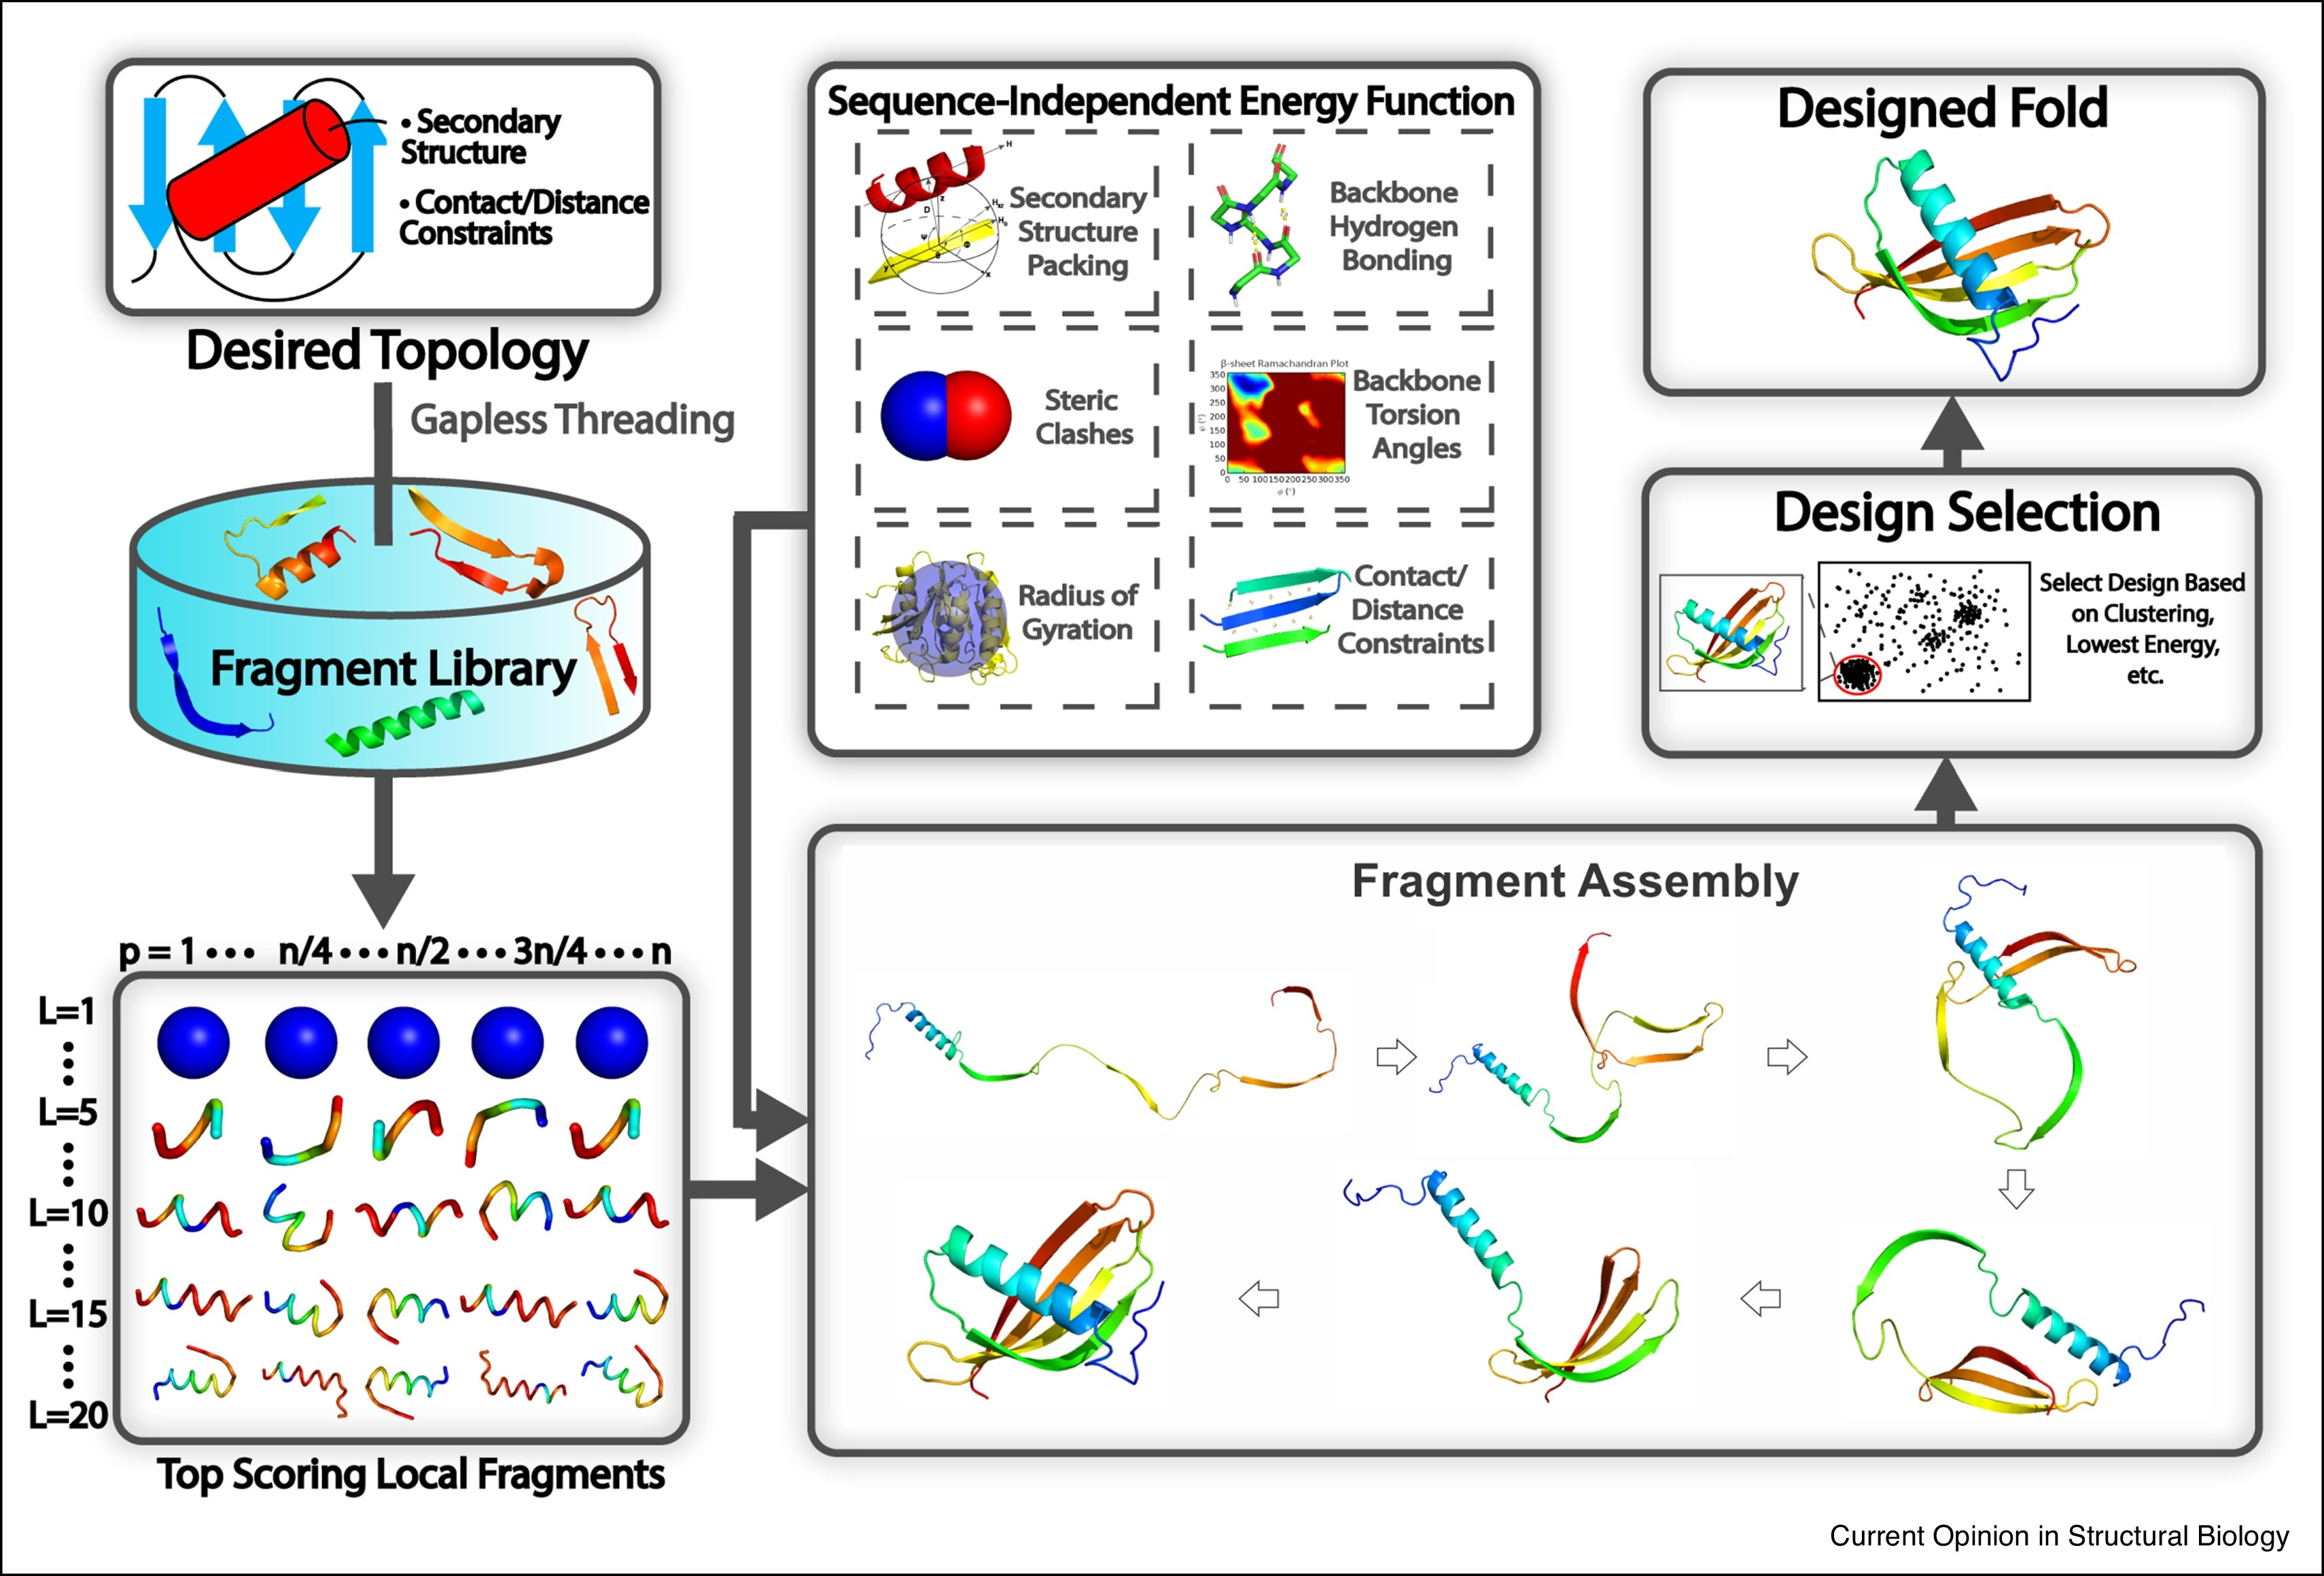
\includegraphics[scale=0.95]{images/fragment-assembly.jpg}
	\caption{. Fonte\cite{pearce2021deep}}
	\label{fig:fragment-assembly}
\end{figure}

Typical steps involved in a fragment assembly based approach to design new protein structures. Starting from the desired secondary structure together with user-defined packing restraints, such as residue⿿residue contact/distance restraints, the query is searched through a non-redundant PDB structure library using gapless threading to generate position-specific fragment structures. High scoring fragments, which may range from 1 to 20 residues long, are identified based on the complementarity between the desired secondary structure and a fragment⿿s secondary structure and backbone torsion angles. Then during the folding simulations, the top scoring local fragments are assembled under the guidance of a sequence-independent energy function, which accounts for fundamental rules that govern protein folding such as secondary structure packing, backbone hydrogen bonding, favorable backbone torsion angles, steric clashes, radius of gyration, as well as the artificial contact/distance restraints supplied by the user. As the method is sequence independent, generic side-chain centers of mass, typically those for valine, are used to evaluate energy terms such as steric clashes. Following the folding simulations, the final design may be selected based on clustering of the simulation decoys, by selecting the lowest energy structure, or through whatever filter the user deems appropriate.

The same sorts of genetic engineering techniques can also be employed
to produce new proteins and enzymes that contain novel structures or
perform unusual tasks: metabolizing toxic wastes or synthesizing life-
saving drugs, for example. Most synthetic catalysts are nowhere near as
effective as naturally occurring enzymes in terms of their ability to speed
the rate of selected chemical reactions. But, as we continue to learn more
about how proteins and enzymes exploit their unique conformations to
carry out their biological functions, our ability to make novel proteins
with useful functions can only improve. \supercite{alberts}

\subsection{PSP e Covid-19}

\subsection{Considerazioni sui limiti di AlphaFold}

\subsection{Troppo data-centric?}